\subsection{Soil Desiccation}
\subsectioncover

\begin{frame}
  \vspace{-1.5em}
  \begin{columns}[T]
    \begin{column}{0.5\textwidth}
      \begin{figure}
        \centering
        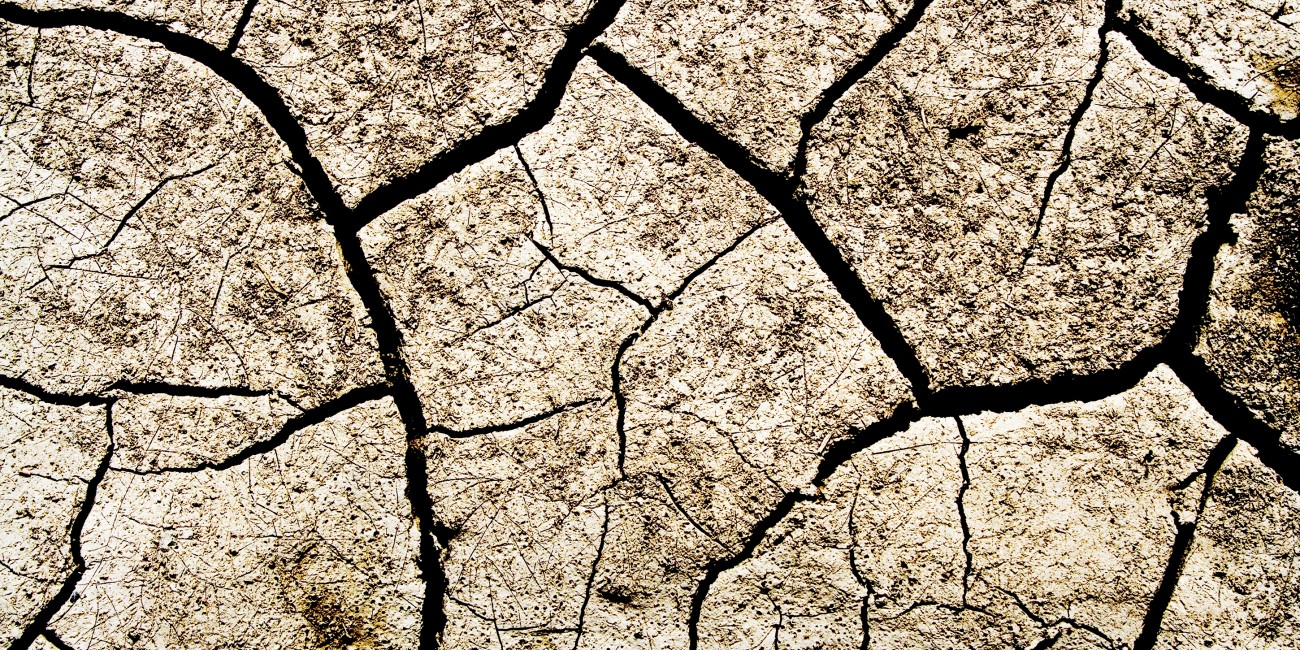
\includegraphics[width=0.7\textwidth]{Chapter1/figures/desiccation}
      \end{figure}
      
      Background:
      \begin{itemize}
        \item Film-substrate systems widely exist in nature and in engineering applications.
        \item Fracture of thin films has been studied using model-based simulations based on a wide range of methodologies.
        \item Many soil materials are ``cohesive'' in nature. It calls for a phase-field model for cohesive fracture.
        \item Many film-substrate systems are symmetric or axisymmetric. It is important to incorporate stochastic models for material properties.
      \end{itemize}
    \end{column}
    \begin{column}{0.5\textwidth}
      Model:
      \begin{itemize}
        \item Enforcing traction-free boundary conditions:
              \begin{align*}
                 & \psi^e = g\psi^e_\activepart + \psi^e_\inactivepart ,                                                                                  \\
                 & \psi^e_\activepart = \dfrac{1}{2}\stress_\activepart:\strain, \quad \psi^e_\inactivepart = \dfrac{1}{2}\stress_\inactivepart:\strain , \\
                 & \stress_\activepart = \stress_n^+ + \stress_t, \quad \stress_\inactivepart = \stress_n^-,                                              \\
                 & \stress_n^\pm = \macaulay{-t_N}_\pm\xnormal\otimes\xnormal, \quad  \stress_t = \stress - \stress_n^+ - \stress_n^-.                    
              \end{align*}
        \item Cohesive fracture:
              \begin{align*}
                 & \alpha = \xi d- (1-\xi) d^2, \quad g = \dfrac{1}{1+\phi}, \\
                 & \phi = \dfrac{a_1d + a_1a_2d^2 + a_1a_2a_3d^3}{(1-d)^p}.  
              \end{align*}
        \item A nonlinear softening law:
              \begin{align*}
                \xi = 1, \quad p = 2, \quad a_1 = \dfrac{\Gc}{c_0 l \psi_c}, \quad a_2 = 1, \quad a_3 = 0.
              \end{align*}
      \end{itemize}
    \end{column}
  \end{columns}
\end{frame}

\begin{frame}
  \vspace{-1.5em}
  \begin{columns}[T]
    \begin{column}{0.6\textwidth}
      \vspace{-1em}
      \begin{figure}
        \centering
        \begin{subfigure}{0.32\linewidth}
          \centering
          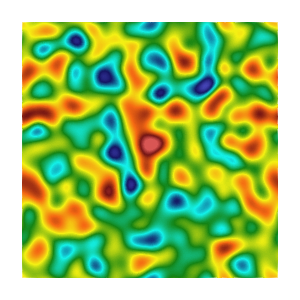
\includegraphics[width=0.8\textwidth]{Chapter345/figures/Gc_sqexp_cartesian_5_5_rho_0_seed_a}
        \end{subfigure}
        \begin{subfigure}{0.32\linewidth}
          \centering
          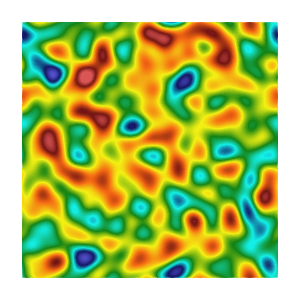
\includegraphics[width=0.8\textwidth]{Chapter345/figures/psic_sqexp_cartesian_5_5_rho_0_seed_a}
        \end{subfigure}
        \begin{subfigure}{0.32\linewidth}
          \centering
          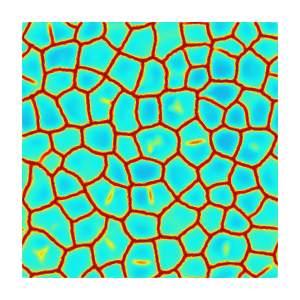
\includegraphics[width=0.8\textwidth]{Chapter345/figures/d_sqexp_cartesian_5_5_rho_0_seed_a}
        \end{subfigure}
        
        \begin{subfigure}{0.32\textwidth}
          \centering
          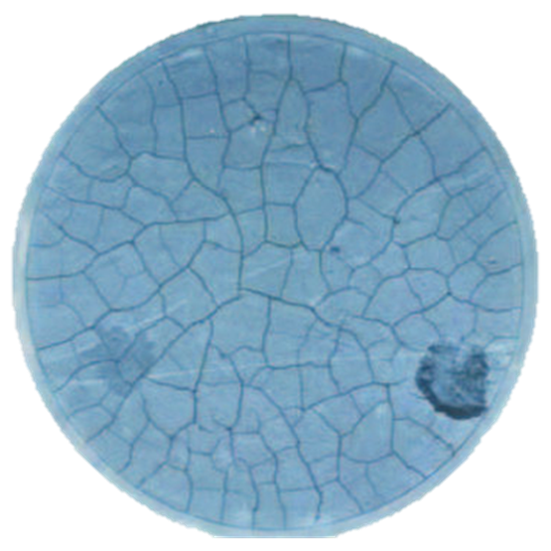
\includegraphics[width=0.8\textwidth]{Chapter345/figures/4mm_exp.png}
        \end{subfigure}
        \begin{subfigure}{0.32\textwidth}
          \centering
          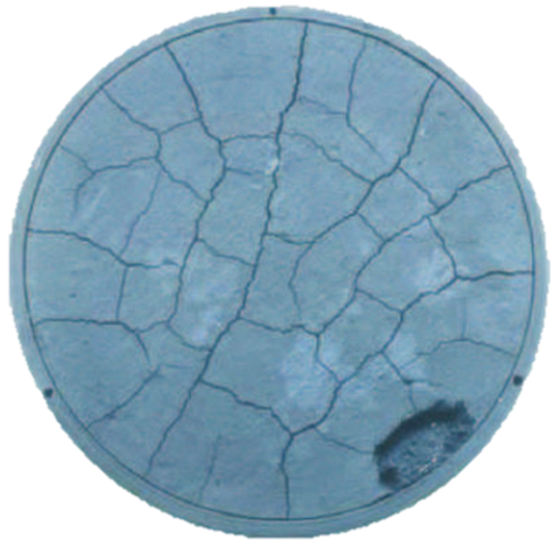
\includegraphics[width=0.8\textwidth]{Chapter345/figures/8mm_exp.png}
        \end{subfigure}
        \begin{subfigure}{0.32\textwidth}
          \centering
          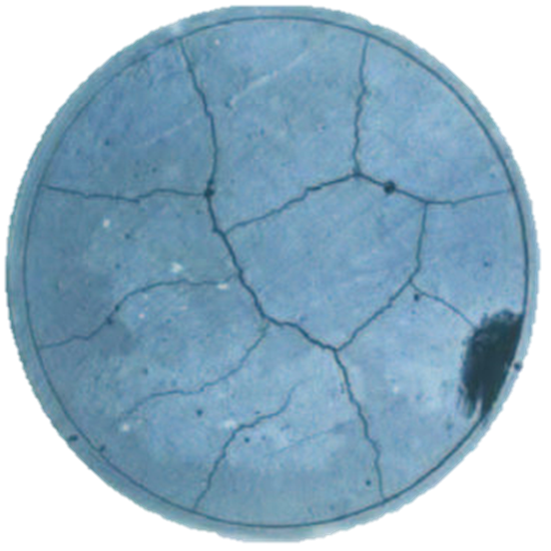
\includegraphics[width=0.8\textwidth]{Chapter345/figures/16mm_exp.png}
        \end{subfigure}
        
        \begin{subfigure}{0.32\textwidth}
          \centering
          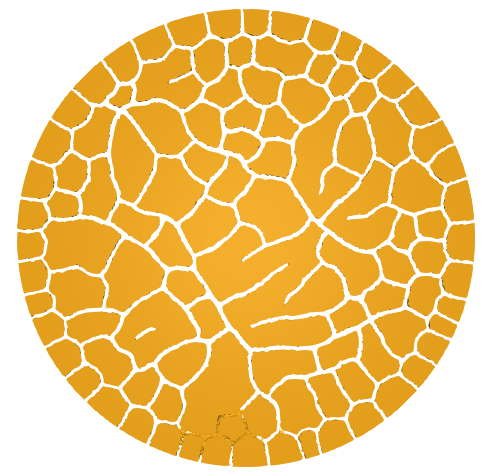
\includegraphics[width=0.8\textwidth]{Chapter345/figures/4mm_top.png}
        \end{subfigure}
        \begin{subfigure}{0.32\textwidth}
          \centering
          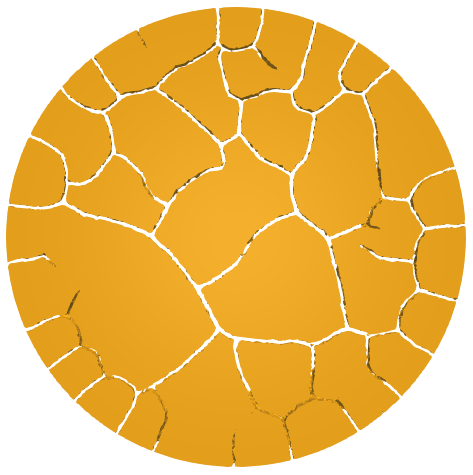
\includegraphics[width=0.8\textwidth]{Chapter345/figures/8mm_top.png}
        \end{subfigure}
        \begin{subfigure}{0.32\textwidth}
          \centering
          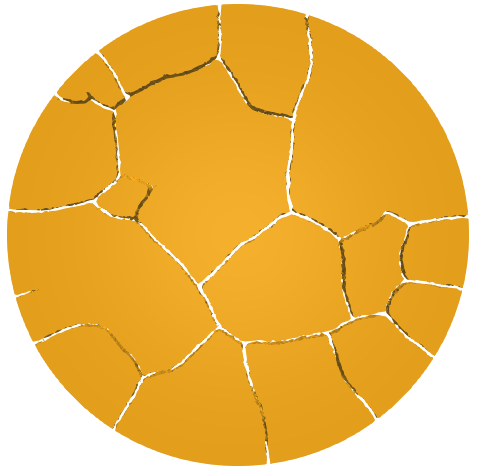
\includegraphics[width=0.8\textwidth]{Chapter345/figures/16mm_top.png}
        \end{subfigure}
      \end{figure}
    \end{column}
    \begin{column}{0.4\textwidth}
      \begin{itemize}
        \item Only ``channeling'' cracks in the thin film are considered.
        \item Thermal effects are neglected. Dehydration is modeled as pre-stress (or equivalent eigenstrains).
        \item The fracture model is verified with analytical solutions in a periodic quasi-1D context.
        \item Pervasive fracture is studied with a 2D simplification.
        \item Material property inhomogeneity is represented by two pointwise correlated random fields $\{\Gc(\bs{X}), \bs{X} \in \body\}$ and $\{\psi_c(\bs{X}), \bs{X} \in \body\}$.
        \item The versatility offered by the probabilistic framework is highlighted by solving a 3D problem based on physical experiments.
      \end{itemize}
    \end{column}
  \end{columns}
\end{frame}
